\chapter[Extension: Eye-movement control and parsing]{An extension of the core model: 
Modelling the interaction of eye-movement control and parsing} \label{c02emma}

\section{Introduction}
In language comprehension research, most of the evidence about the cognitive processes involved comes from the study of eye movements in reading.  As the reader's eyes move through a sentence, the  sequence of fixations and their durations reflect the reader's allocation of attention and the processing effort necessary to combine the words incrementally into a coherent structure.  The specific linking between fixation patterns and the underlying cognitive processes is, however, not trivial: Fixations are determined not only by immediate low-level processes like word recognition but also by more complex operations such as structural parsing decisions, contextual integration, and non-linguistic oculomotor constraints.  In recent years, a number of computational models have emerged that help understanding the reading process in detail \citep{BicknellLevy2010a,EngbertEtAl2002,Engbert2005,Legge2002,Reichle1998,Nilsson2010,Reichle2006,Reilly2006}.  
The two most developed models of this kind are \index{E-Z Reader} E-Z Reader \citep{Reichle2006} and \index{SWIFT} SWIFT \citep{Engbert2005}.  These generate predictions based on \index{lexical variables} lexical variables like word frequency, word length, and cloze predictability.  Although they differ fundamentally in their core assumptions about the nature of the reading process (E-Z Reader shifts attention \index{serial word processing} serially while SWIFT allows for \index{parallel word processing} parallel word processing guided by an attentional gradient), both models make very accurate predictions about when and where the eyes move.  However, since these models rely on word-level information, their predictions are limited to rather simple sentences that do not induce severe interruptions of the reading process.\footnote{This chapter is reused  with permission from \cite{Engelmanna}, Copyright (2013) Wiley; license number 4740811363588.}

Postlexical processes \index{postlexical processes} like structural and semantic integration operate on a higher level and can only be uncovered by studying more complex sentences that contain long-range dependencies, ambiguities, or contextual inconsistencies.  Challenging the sentence processor in this way reveals memory operations, structural and semantic predictions, and repair processes.
In particular, there has been an abiding interest in identifying spatio-temporal distributions of short- and long-range regressions (backward saccades) in psycholinguistic literature \cite{vanDyke2003,Frazier1982a,MalsburgVasishth2011,MalsburgVasishth2012,Meseguer2002,MitchellEtAl2008,Weger2007}. 
In most established eye movement models, however, inter-word regressions are caused either by incomplete lexical processing (e.g., SWIFT) or due to motor error (e.g., older versions of E-Z Reader).  An exception is the model of \cite{BicknellLevy2010a}, which explains regressions as the result of a rational strategy guided by Bayesian inference on the sentence level. 
The postlexical level of sentence processing has been captured by a range of computational models \citep{Binder2001,Elman:2005p2,Hale2011,JustCarpenter1992,Konieczny2003,Budiu2004,LewisVasishth2005,MacDonaldChristiansen2002,SpiveyTanenhaus1998,VasishthBruessowLewis2008}.  These models predict word-by-word difficulty, which can be correlated with aggregated eyetracking measures but abstracts away from individual fixations.

In order to understand how postlexical difficulty and eye movements interact, it is necessary to combine both classes of computational models and investigate the link between high-level language processes and oculomotor control.  In a recent approach, \cite{ReichleWarrenMcConnell2009} introduced a postlexical integration stage into E-Z Reader 10, that interacts with eye movement control through regressions.  Whenever the integration stage takes too long, a regression is triggered in order to buy time for the integration process to finish.  Although Reichle and colleagues did not integrate a computational account of postlexical processing, they showed a suitable way toward studying the link between parsing and eye movements.

In the work presented here, the cognitive architecture ACT-R \citep{AndersonEtAl2004} is used to combine an eye movement control model with a parser in a similar way as \cite{ReichleWarrenMcConnell2009} did. However, we incorporate two well-tested computational accounts of parsing difficulty that capture \index{memory retrieval} memory retrieval and \index{structural prediction} structural prediction, respectively: (1) The syntactic retrieval account of \cite{LewisVasishth2005} builds on independently motivated assumptions about memory access and has been implemented as a fully specified parser in ACT-R; (2) Surprisal \cite{Hale2001,Levy2008} defines difficulty in terms of disconfirmed structural predictions.
The combination of both metrics in one model is motivated by empirical evidence and statistical modelling: Experimental results suggest a complementary relation between expectation-based and working-memory-based accounts \citep{Demberg2008,Konieczny2000,Vasishth2011,Staub2010a}, and corpus studies show that surprisal and retrieval are independent predictors of processing difficulty \citep{Boston2008,BostonHaleVasishth2011,Patil2009,VasishthLewis2006}. 
The use of ACT-R has several advantages. First, ACT-R implements cognitive principles that are valid in distinct domains and enables the development of models for various tasks. Second, it integrates all levels of cognition from visual and motor processes that interact with a virtual outside world to rule-based reasoning.  Third, ACT-R is a model of real-time processing, which makes its predictions directly comparable to eyetracking data in milliseconds.
As an eye-movement control model we use the ACT-R-integrated EMMA \index{EMMA}  (``eye movements and movement of attention'') developed by \cite{Salvucci2001}, which is in principle a simplified and domain-independent version of E-Z Reader.

The goal of this paper is to demonstrate the feasibility of integrating a computational account of postlexical difficulty with an eye movement control model.  For that purpose we avail ourselves of a framework which is simplifying in some respects but exhibits enough flexibility for further development and extension.  In order to provide a general assessment which is comparable to earlier studies \citep{Reichle1998,ReichleWarrenMcConnell2009,Salvucci2001}, we perform a qualitative examination of the framework on a suitable eyetracking corpus.  Although E-Z Reader and EMMA were evaluated on the Schilling Corpus \cite{Schilling1998}, we used the German Potsdam Sentence Corpus \cite{Kliegl2004} because measures of parsing difficulty are readily available for the latter.
Section 2 will introduce EMMA in detail.  In Section 3, we present a replication of \cite{Salvucci2001} on the English Schilling Corpus, which is necessary because ACT-R has developed further since Salvucci's evaluation of EMMA in 2001, and EMMA itself has been re-implemented.  The successful replication provides the basis for an extension of the model with parsing theory which will be described in Section 4.  Finally, Section 5 presents six simulations on the German Potsdam Sentence Corpus that assess a range of model configurations that integrate EMMA with surprisal and retrieval.

\section{The EMMA/ACT-R reading model}
EMMA's basic assumptions were inspired mainly by E-Z Reader. The main characteristics of the model are a dynamic calculation of word encoding time and a distinction between overt eye movements and covert shifts of attention. Attention is allocated serially and proceeds usually ahead of the eye movement. This enables the model to produce skipping and refixations. The programming of saccades consists of a labile stage, i.e., a stage that can be canceled by upcoming attention shifts, and a non-labile state, after which the saccade preparation has passed a point of no return leading to an eye movement inevitably. Below we describe the version of EMMA that we used for our simulations in the environment of ACT-R 6.0.

The core function of EMMA calculates the encoding time of an object based on its frequency of occurrence and its eccentricity from the current viewing location. The resulting duration represents attention shift and word identification in one step. The encoding time $T_{enc}$ is calculated in the following way:
\begin{equation}
T_{enc} = K (- \log{f_i}) e^{k\epsilon_i}
\end{equation}
where $K$ (visual encoding factor) and $k$ (encoding exponent) are scaling constants, $\epsilon_i$ is the eccentricity of the object ($i$) to be encoded, and $f_i$ is the object's corpus frequency normalized to a range between 0 and 1 (word occurrence per one million words divided by one million). The saccade preparation time $T_{prep}$ has been estimated in Salvucci's simulations to 135~ms.\footnote{In ACT-R 6.0, the planning time for motor processes amounts to 0, 50, 100, or 150~ms depending on feature-based similarity with the previous movement. However, for our simulations we used Salvucci's original definition of a fixed preparation time.} The non-cancelable stage $T_{exec}$ consists of 50~ms for saccade programming, 20~ms for saccade execution and additional 2~ms per degree of visual angle of the saccade length. The model introduces variability to $T_{enc}$, $T_{prep}$, and $T_{exec}$ by randomly drawing from a uniform distribution\footnote{A uniform distribution is the ACT-R 6.0 default for random time generation. In Salvucci's original model a Gamma distribution was used.} with a standard deviation of one third of the actual value. Also, landing point variability of a saccade is defined by a Gaussian distribution with a standard deviation of 0.1 times the intended saccade distance. For empirical motivations for the choice of distributions, see \cite{Salvucci2001}.

Salvucci presented three evaluations of his EMMA/ACT-R model on empirical data from equation-solving, visual search, and reading. In the case of reading, which is the application of interest here, EMMA was interfaced with a simple ACT-R model that worked in the following way: Each cycle begins with the initiation of an attention shift to the nearest object to the right. EMMA then initiates the encoding of the target object using the provided frequency values and, at the same time, starts the preparation of the corresponding eye movement. Once the visual encoding has finished, the model performs a lexical retrieval of the input word and starts the next cycle by shifting attention to the next word. The lexical retrieval had a fixed duration and, thus, did not contribute to the predictions in a relevant way.
Salvucci tested EMMA on the 48 sentences of the Schilling Corpus \citep{Schilling1998} and showed that the model reproduced well-known empirical effects of word-frequency on a range of eyetracking measures.

%%%%%%%%%%%%%%%%%%%%%%%%%%%%%%%%%%%%%%%%%%%%%%%%%%%%%%%
%%% S1: SRC
%%%%%%%%%%%%%%%%%%%%%%%%%%%%%%%%%%%%%%%%%%%%%%%%%%%%%%%
\section{Replication of Salvucci (2001)}
\subsection{Data}
The Schilling Corpus (SC) contains fixation data of 48 American English sentences with 8-14 words each, read by 48 students.
For evaluating the model performance, \cite{Salvucci2001} used data compiled by \cite{Reichle1998}. They had calculated the means of six eyetracking measures for five logarithmic frequency classes (see Table \ref{classtable}). The frequency values available in the SC were obtained from \cite{Francis1982}.  In order to avoid confounds, the first and the last word of each corpus sentence was removed. Since the model did not produce regressions, trials that contained inter-word regressions (64\%) were excluded from the analysis.  

\begin{table}[!htbp]
\centering
\begin{tabular}{crrrrrr} 
%\toprule
\hline
  &  & \multicolumn{2}{c}{SC} & & \multicolumn{2}{c}{PSC} \\ \cline{3-4} \cline{6-7}
  Class & Freq. in 1M & Words & Mean & & Words & Mean   \\ 
%\midrule
\hline
  1     & 1--10   & 77  & 3     & & 186 & 3         \\
  2     &  11--100 & 87  & 50    & & 173 & 41        \\
  3     &  101--1000 & 71  & 333   & & 200 & 335       \\
  4     &  1001--10,000 & 92  & 5067  & & 207 & 5020      \\
  5     &  $>$10,000  & 112 & 41976 & & 84  & 2399      \\ 
%\bottomrule
\hline
\end{tabular}
\caption{Frequency classes used in the analyses of the Schilling Corpus (SC) and Potsdam Sentence Corpus (PSC).}
\label{classtable}
\end{table}

\subsection{Model}
Our ACT-R model consisted of four productions: \index{find-next-word} \texttt{find-next-word} (search for the nearest object to the right), \index{attend-word} \texttt{attend-word} (initiate an attention shift and encoding by EMMA), \index{integrate-word} \texttt{integrate-word} (start memory retrieval), and \index{stop-reading} \texttt{stop-reading} (when the sentence is finished).  The \texttt{integrate-word} rule did not do anything in this model apart from adding 50~ms to the processing time. It was used in later simulations, however, to initiate the parsing process.
All simulations presented here were carried out in ACT-R 6.0. We used EMMA version 4.0a1 (with some minor adjustments by us) as it has been re-implemented by Mike Byrne and Dan Bothell in order to be fully integrated in ACT-R 6.0.  All parameters except for those shown in Table~\ref{simtable} were kept at their default values.  This is particularly important for the \emph{default action time}, which is the firing duration assigned to each ACT-R production rule. \cite{Salvucci2001} set it to 10~ms, but in ACT-R 6.0 it defaults to 50~ms.

\begin{sidewaystable}[!htbp]
\centering
\begin{tabular}{lllrrrrrrrrr}
%\toprule
\hline
 & & & \multicolumn{4}{c}{Parameters} & & \multicolumn{3}{c}{Fit} & \\ \cline{4-7} \cline{9-11}
% latex table generated in R 2.15.2 by xtable 1.7-0 package
% Tue Nov 27 13:22:28 2012
  &   &   & $K$ & $T_{prep}$ & $F$ & $P$ &   & $R_{early}$ & $R_{late}$ & $RMSD$ & $\%reg$ \\ 
 % \midrule
 \hline
no regr. &  & Salvucci (2001) & 0.006 & 0.135 &  &  &  & 0.97 &  & 0.362 & 0 \\ 
   & 1 & SC replication & 0.002 & 0.135 &  &  &  & 0.96 &  & 0.303 & 0 \\ 
   & 2a & PSC & 0.003 & 0.120 &  &  &  & 0.86 &  & 0.326 & 0 \\ 
 % \midrule
 \hline
PSC all & 2b & EMMA & 0.003 & 0.120 &  &  &  & 0.91 & 0.38 & 0.638 & 0 \\ 
   & 3 & +s$_1$ & 0.002 & 0.115 &  & 0.0030 &  & 0.93 & 0.39 & 0.645 & 0 \\ 
   & 4 & +r & 0.002 & 0.110 & 0.2 &  &  & 0.90 & 0.86 & 0.201 & 18 \\ 
   & 5 & +s$_2$ & 0.003 & 0.115 &  & 0.0200 &  & 0.92 & 0.87 & 0.229 & 15 \\ 
   & 6 & +rs$_1$ & 0.003 & 0.115 & 0.2 & 0.0005 &  & 0.92 & 0.88 & 0.257 & 12 \\ 
   & 7 & +rs$_2$ & 0.003 & 0.115 & 0.1 & 0.0150 &  & 0.90 & 0.91 & 0.206 & 23 \\
 \hline 
%\bottomrule
\end{tabular} \\ 
\footnotesize{
\emph{Notes:} $K$ = EMMA encoding factor, $T_{prep}$ = EMMA saccade preparation time, $F$ = ACT-R retrieval latency factor, $P$ = scaling factor for surprisal. The fit was calculated for means of 5 frequency classes for each eyetracking measure. $R_{early}$ = correlation coefficient between observed and predicted values for early measures (gaze, FFD, SFD, skip, onefix, and refix). $R_{late}$ = correlation coefficient for late measures (RPD, TFT, RRT, FPREG, and reread). The last two columns show the total normalized root-mean-square deviation and the percentage of simulated trials that contained regressions.}
\caption{Fit and parameter estimates for all simulations.}\label{simtable}
\end{sidewaystable}

\begin{figure}[!htbp]
\begin{center}
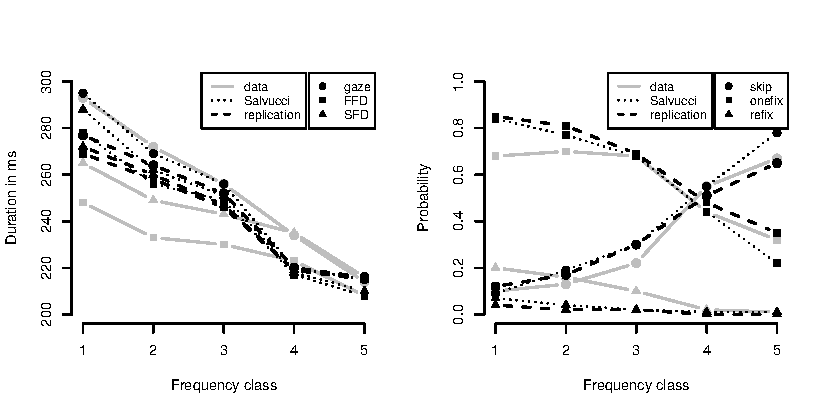
\includegraphics[width=0.8\textwidth]{figures/fig-src-fstat}
\end{center}
\caption{Replication of Salvucci (2001) on the Schilling Corpus. Effects of word frequency on gaze, first, and single fixation duration, and on the rate of skipping a word, fixating it once and fixating it more than once.  Grey solid lines represent experimental data, black dotted lines show Salvucci's simulation results, and black dashed lines show the replication results.  Lexical frequency is divided into classes 1 (lowest) to 5 (highest).}
\label{fig:src-fstat}
\end{figure}

\subsection{Analysis}
One simulation consisted of 10 complete model runs through the 48 sentences of the Schilling Corpus.  Fixations times were recorded for each word.  The analysis was carried out in the R{} statistics software \cite{R2012}.  Following the analysis of \cite{Reichle1998} and \cite{Salvucci2001}, we excluded first and last words from the sentences and all trials that contained inter-word regressions. Then we divided the corpus words into five logarithmic frequency classes (see Table \ref{classtable}) and calculated the means for each class for six fixation measures: gaze duration (the time spent on a word during first pass, including immediate refixations), first fixation duration (FFD, duration of the first fixation on a word during first pass), single fixation duration (SFD, fixation duration on a word if it is fixated only once during first pass), the skipping rate of a word (skip), the probability of fixating a word exactly once (onefix), and the probability of fixating a word more than once (refix).  This analysis was done with both the experimental data and the model output.
We quantified the goodness of fit between the model predictions and the data using the  \emph{Pearson product-moment correlation coefficient} $R$, and the \index{root-mean-square deviation} \emph{root-mean-square deviation} ($RMSD$).  $RMSDs$ were normalized by the standard deviation of the observed data in the same way as it was done in \cite{Reichle1998} and \cite{Salvucci2001}.  A precise definition is given in the Appendix.
The parameter optimization procedure was carried out by first identifying a number of parameter configurations with $R$ values near the maximum and then, among these, choosing the one with the smallest $RMSD$.  In this way, the optimization represented a priority for the quality of effects while also taking quantity into account.

\subsection{Results}
We re-estimated the encoding factor $K$ and the saccade preparation time $T_{prep}$ in order to compensate for the changes in the ACT-R environment.  See Table~\ref{simtable} for a summary of the simulation results including estimated parameter values.  
The parameter fitting resulted in a decrease of $K$, which should mainly be due to the increased default action time of 50~ms in ACT-R 6.0.
Fig. \ref{fig:src-fstat} shows the predictions of the model (dashed lines) for six fixation measures as a function of frequency class.  Besides the corpus data (grey solid lines), we also plotted the results of the original study (dotted lines) as reported in \cite{Salvucci2001} for comparison.
The main trends in the data are that high-frequency words are read faster and skipped more often than low-frequency words. These trends and the overall pattern of the data were reproduced by the model with a close fit to the original predictions. The mean correlation $R$ with the data was 0.96 and the mean $RMSD$ was 0.303.

\subsection{Discussion}
The EMMA/ACT-R model, as re-implemented in ACT-R 6.0, reproduces frequency effects on fixation durations and probabilities in the Schilling Corpus with a performance comparable to that of the original simulation of \cite{Salvucci2001}.  Despite the different environment, a small adjustment to the encoding time was sufficient to replicate the results.  
The successful re-evaluation of EMMA in its current version is essential for the next steps that will extend the model with accounts of parsing theory.

\section{The extended EMMA/ACT-R model}
In order to augment the EMMA/ACT-R model with postlexical processing, we take a similar approach as \cite{ReichleWarrenMcConnell2009}.  The integration stage of E-Z Reader 10 operates in parallel to eye movement control but can interrupt the reading process for two reasons: Either integration of a word $w_n$ just fails (``rapid integration failure'') or the integration process takes too long (``slow integration failure''), which means that the integration of word $w_n$ does not finish before the identification of word $w_{n+1}$ is completed.
In either case, the eyes are directed back to word $w_n$ or $w_{n-1}$ with a certain probability.  
Reichle and colleagues demonstrated the applicability of their model by re-configuring the model parameters for three cases of parsing difficulty: clause wrap-up, semantic violations, and garden paths. 

Our goal is to evaluate a model which works in a similar way but uses a computational implementation of sentence comprehension to generate its predictions. 
Since in ACT-R only one retrieval request can be handled at a time, it follows naturally that retrieval of word $w_{n}$ has to be completed before the integration of word $w_{n+1}$ can start.  Once initiated, retrieval operates in parallel to cognition and eye movement planning. As long as the difficulty is low and retrieval completes fast, the reading process is uninterrupted.  The possibility that retrieval fails completely (rapid integration failure) is not included in the model for now.
Similar to E-Z Reader 10, when identification of word $w_{n+1}$ finishes before the complete integration of word $w_n$, our model initiates a regression back toward the previous word.  Once word integration is complete, the model continues with normal reading.  This type of regressions has been proposed by \cite{MitchellEtAl2008}.  They called them \index{time-out regressions} ``Time Out regressions'' because their assumed function is to provide additional time for the sentence processor before taking up new input.

The above described concept of interrupting the ``normal'' reading process by time outs should not be misunderstood in the way that making regressions is not normal.  We assume that these interruptions by the parser belong to normal reading as they happen quite regularly and are not under conscious cognitive control.  A quite different case are active reanalysis mechanisms where the reader is aware of an inconsistency (syntactic or semantic) and has to make long-range regressions.  However, although the presented framework can be used to study this kind of behavior, we restrict our study to the simplest case for now.

For simulating postlexical processing, we use two complementary explanations of parsing difficulty: cue-based retrieval \citep{LewisVasishth2005} and \index{syntactic surprisal} syntactic surprisal \citep{Hale2001,Levy2008}. 

\subsection{Retrieval}
In sentence processing, in order to create structural dependencies (e.g., between verbs and their arguments), items in memory have to be accessed; the success and duration of these access events are modulated by, inter alia, the distance between the dependents and the amount of interference from other items \citep{Just1980,JustCarpenter1992,Gibson2000,grodner,Bartek2011}.
\cite{LewisVasishth2005} developed a computational model of parsing difficulty that adopts ACT-R's memory principles of fluctuating activation, decay over time, and similarity-based interference.  The model was implemented in ACT-R as a fully-specified left-corner parser that incrementally builds a structural representation, following X-bar rules. The constituents of the tree structure are stored as \emph{chunks} in ACT-R's declarative memory (related to each other by features like specifier, comp, and head).  In order to integrate an input word into the current structure, the parser carries out the following steps: (1) Access the corresponding lexical entry in the lexicon in declarative memory; (2) Based on syntactic expectations, specify the features of a matching constituent and initiate a retrieval; (3) Create a new syntactic constituent and attach it to the one retrieved.
Using the model's predictions of parsing duration, \cite{LewisVasishth2005} explained effects of distance and structural interference in sentence processing in terms of independently motivated principles of working memory access.  The retrieval model has found further applications in accounts of anti-locality \citep{VasishthLewis2006}, negative polarity constructions \citep{VasishthBruessowLewis2008}, reflexive binding \citep{PatilVasishthLewis2016}, and impaired sentence comprehension in aphasia \citep{PatilEtAl2016}.

To summarize, the sentence processing model of \cite{LewisVasishth2005} is a fully-specified parser the actions of which can be transparently measured in milliseconds. It relies on domain-independent memory principles,  and it is well-tested by a number of applications.  This kind of model is exactly what is needed in order to investigate the interaction between parsing and eye movements in detail. We connect this parsing model to EMMA via Time Out regressions. 


\subsection{Surprisal}
\index{surprisal}
Surprisal \citep{Hale2001,Levy2008} formalizes the idea that unexpected structures cause processing difficulty \citep{Konieczny2000}. \cite{Hale2001} defined the surprisal of a word as a function of the probability mass of all derivational options that have to be disconfirmed at that point in the sentence.
The surprisal of a word $w_i$ is the negative logarithm of the transition probability from word $w_{i-1}$ to $w_i$. The lower the probability of a word given its preceding context, the higher its surprisal. While Hale assumed a complete knowledge of the grammar to define the surprisal value, there are also different accounts of calculating surprisal, e.g., using a neural network \citep{Frank2009} or using a rationally bounded parallel dependency parser \citep{BostonHaleVasishth2011}.

Although the difficulty associated with surprisal stems from building low-probability structures, it is not clear that the cause of the difficulty must be located in postlexical processing.
Given the conceptual distinctness of surprisal and retrieval together with experimental evidence locating expectation effects earlier than memory effects \citep{Staub2010a,Vasishth2011}, we hypothesize that the source of these two types of difficulty may lie at different points in the processing time course.
Theoretically, it is legitimate to assume that the contextually pre-activated high-probability structures (or parsing steps) would also pre-activate lexical items belonging to the according categories. In that case, at every point in the sentence the activation of specific lexical items receives a boost by its structural context. This would directly affect the speed of the word identification process.
That means, although the source of surprisal difficulty is undoubtedly a ``high-level'' postlexical process, the actual realization of that difficulty could happen ``low-level'' at the stage of word identification.

The following simulations test both assumptions, surprisal affecting the \index{high-level surprisal} high-level and affecting the \index{low-level surprisal} low-level.  The high-level variant is implemented by additively modulating the duration of the integration stage by a scaled surprisal value. For simulating surprisal affecting the low-level we include the surprisal values in EMMA's core equation of word encoding time. The resulting equation for $T_{enc}$ will be shown in the next section.

\section{Simulations on the Potsdam Sentence Corpus} \label{sec:topics:psc}

\index{Potsdam Sentence Corpus}
In this section, we present six simulations that were carried out on the Potsdam Sentence Corpus (PSC) developed by \cite{Kliegl2004}. The PSC was used because \cite{Boston2008} and \cite{BostonHaleVasishth2011} provide retrieval and surprisal values for all corpus words.  Simulation 2 evaluated EMMA on the PSC in order to compare the results with the model performance on the Schilling corpus.  Besides assessing how well the model can be generalized to another corpus in a different language, this study pursued the goal to establish the basis for augmenting the EMMA/ACT-R model with postlexical processing. 
The other five simulations tested EMMA in different configurations that include and combine retrieval (r), low-level surprisal (s$_1$), and high-level surprisal (s$_2$): EMMA+s$_1$, EMMA+r, EMMA+s$_2$, EMMA+rs$_1$, and EMMA+rs$_2$ (see Table \ref{simtable} for an overview).

\subsection{Data}
\paragraph{Potsdam Sentence Corpus}
The Potsdam Sentence Corpus contains eyetracking data from 144 simple German sentences (1138 words) with 5 to 11 words per sentence, read by 229 readers. 
The corpus contains values of printed word frequency obtained from the \index{CELEX database} CELEX database, a corpus of about 5.4 million words \citep{Baayen1993}.
\cite{Kliegl2004} report effects of frequency on reading times and probabilities using the same logarithmic frequency classes that were used in \cite{Salvucci2001} (see Table \ref{classtable}). The trends are comparable to those in the \index{Schilling Corpus} Schilling Corpus: Higher frequency correlates with shorter reading times and higher skipping rates, although the trend is not as strong in first and single fixation durations. 

We integrated retrieval and surprisal information in the corpus data that provided the input for the EMMA/ACT-R model.

\paragraph{Retrieval}
There are handcrafted ACT-R parsing rules available for a number of psycholinguistically interesting sentence constructions;  however, not enough to cover the whole PSC.  For this corpus-based benchmarking evaluation carried out here, we therefore used pre-calculated values from \cite{BostonHaleVasishth2011}.  These retrieval values were calculated using a parallel dependency parser and approximately represent the duration a retrieve-and-attach cycle would require in the ACT-R parser.  Each step of the dependency parser (\texttt{SHIFT}, \texttt{REDUCE}, \texttt{LEFT}, \texttt{RIGHT}) was assigned a duration of 50 ms --- the \emph{default action time} in ACT-R that it takes one production to fire.  The duration of retrieving an item from memory was calculated using ACT-R equations, including a simplified version of similarity-based interference.  The parser was assessed at different levels of parallelism, i.e., the number of alternative derivations to be pursued at the same time.
The retrieval values obtained at the highest level of parallelism (100 parallel analyses) were the most significant predictors in \cite{BostonHaleVasishth2011}.  These values (M = 357.8~ms, SD = 122.16~ms) were used in our model to imitate the parsing process.  The values were scaled with the ACT-R-internal \index{latency factor} \emph{retrieval latency factor} $F$.

\paragraph{Surprisal}
For the present purposes, we used surprisal values (M = 2.9~bits, SD = 2.06~bits) from \cite{Boston2008}, which were generated with a modified version of the probabilistic context-free phrase-structure parser\footnote{The parser is publicly available at http://nlp.stanford.edu/$\sim$rog/prefixparser.tgz} from \cite{Levy2008}.

\subsection{Model}
For the following simulations, the model used in the replication of \cite{Salvucci2001} was modified in the way described in the previous section.  
After encoding word $w_n$, the \texttt{integrate-word} rule starts the parsing actions and attention is shifted to the next word to the right.  For the current study, the parsing duration was imitated by a timer set to the corresponding retrieval value from \cite{Boston2008} scaled by $F$.  As long as the timer is running, no other word can be integrated.

In order to establish a link between cognition and eye movement control, two ACT-R production rules were added to the model: these are called \texttt{time-out} and \index{exit-time-out} \texttt{exit-time-out}.  Their function is as follows: When integration of word $w_n$ is still in progress while the encoding of word $w_{n+1}$ has already completed, \texttt{time-out} initiates an attention shift to the word to the left of the currently fixated one \index{time-out regression} (Time Out regression).  Once the integration of word $w_n$ has finished, the \texttt{exit-time-out} rule returns the model into the state of normal reading.
For reasons of simplicity, no special assumptions are made about the reading process just after a Time Out regression, except for the fact that word $w_n$ will not need to be integrated again.  However, word $w_{n}$ and $w_{n+1}$ will go through the identification process again after leaving Time Out mode because word encoding is part of every attention shift carried out by EMMA.  A more realistic model would probably not fully re-encode a word already identified.  

Note that a Time Out regression can be initiated from word $w_{n}$ or $w_{n+1}$ depending on how fast the encoding process of word $w_{n+1}$ is in relation to the saccade execution to that word.  The regression always targets the word to the left of the current fixation.  This means, the regression target can either be word $w_{n}$ or  $w_{n-1}$.  However, the preparation of a regression can be canceled before its execution in the case when the integration process completes before the non-cancelable state of motor preparation.  In this case, the time out would show itself in the form of a refixation on $w_{n}$ or $w_{n+1}$.  In case this refixation is also canceled because encoding was fast, a saccade to the next word is planned and the time out only causes an increased fixation duration.

Finally, we included the two versions of surprisal described above.  ACT-R was equipped with a surprisal scaling constant $P$. 
For simulating surprisal at the high level, the values scaled by $P$ were added to the duration of the integration stage in milliseconds.  In order to modulate the low-level word encoding process directly by surprisal, we added surprisal in EMMA's word encoding time equation as shown in Equation \ref{eq:emma+s}:
\begin{equation}
T_{enc} = (K [-\log{f}] + Ps)e^{k\epsilon}
\label{eq:emma+s}
\end{equation}
where $s$ is the surprisal value of the corresponding word, and $P$ is the surprisal scaling constant.

\begin{figure}[!htbp]
\begin{center}
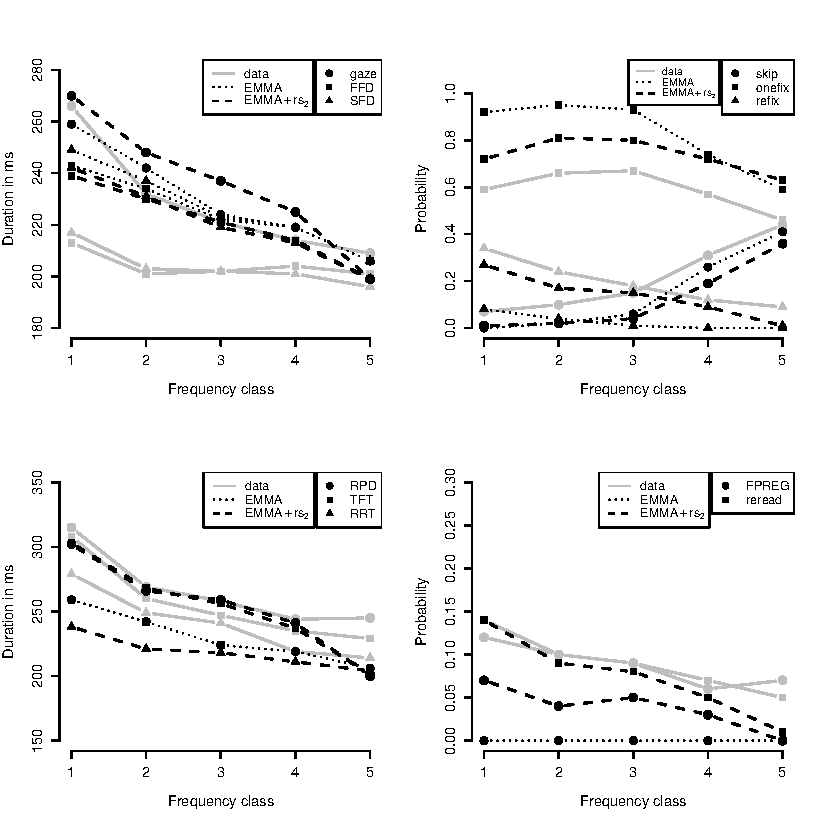
\includegraphics[width=\textwidth]{figures/fig-psc-fstat}
\end{center}
\caption{Shown are the predictions of Model 2 (EMMA, dotted lines) vs. Model 7 (EMMA+rs$\protect  _2$, dashed lines) vs. experimental data (grey solid lines) for the Potsdam Sentence Corpus. The figure shows means of early (first row) and late measures (second row) as a function of frequency class. Each row shows reading time durations on the left and probabilities on the right side.}
\label{fig:psc}
\end{figure}


\subsection{Results}
Simulation results are summarized in Table \ref{simtable}.  Each model was evaluated on the prediction of frequency effects similar to the evaluation of the previous simulation (see Table \ref{classtable} for the frequency classes used in the PSC simulations). However, in addition to the six early fixation measures, we also evaluated the models on the following so-called late measures: \index{regression path duration} regression path duration (RPD, also called go-past duration, the sum of all fixations including previous locations beginning from the first fixation on a word until leaving it to the right), \index{total fixation time} total fixation time (TFT, sum of all fixation on a word), \index{re-reading time} re-reading time (RRT, time spent on a word after leaving it and returning to it), \index{first-pass regression} first-pass regression probability  (FPREG, the probability of regressing from a word in first pass), and the probability of re-reading a word after leaving it to the right (reread).  Note that first-pass regression probability is not literally a late measure.  However, we call it late here because in our model all regressions are caused by late processes.
Except for Simulation 2a, all models were fit and evaluated on the full dataset that contained trials with regressions.  
Like in Simulation 1, the first and the last word of each sentence were excluded from the analysis.  Following the corpus study in \cite{Kliegl2004}, we removed words with first fixation durations longer than 1000 ms and words with gaze and total fixation durations greater than 1500 ms from empirical dataset. This reduced the corpus by a number of 79 words. The results shown in the table were obtained by running 100 iterations on the PSC with the respective parameter sets.
For each model the best fit was determined in the way described in Simulation 1.

\subsubsection{PSC vs. SC}
Simulation 2 was carried out on the PSC using the pure EMMA model without retrieval or surprisal information.
For comparing the model performance on the PSC versus the Schilling Corpus, row 2a in Table \ref{simtable} shows the model performance when trials containing inter-word regressions (40\%) were not considered in the analysis.  For this case, only early measures were compared.  Encoding factor $K$ and $T_{prep}$ were re-estimated.  The predictions have a good correlation with the observed frequency effects ($R_{early} = 0.86$).  Numerically, the predictions deviate more from the data than for the Schilling Corpus, but the $RMSD$ is still reasonable with a value of 0.326.  Note that $RMSD$s are not directly comparable between corpora.  $RMSD$s for the PSC are generally a bit lower because the standard deviations used for normalization are higher than in the Schilling Corpus.

\subsubsection{Influence of parsing difficulty}
In Table \ref{simtable} the PSC simulations are sorted by goodness of fit as defined by the total correlation $R$, which is the mean of $R_{early}$ (correlation for the early measures) and $R_{late}$ (correlation for the late measures).  It shows that the model performance on predicting frequency effects gradually improves through the extension with measures of surprisal and retrieval.
In order to provide a baseline for the EMMA+ ~models, Simulation 2 was analyzed again on the complete dataset including trials that contained regressions (see row 2b). 
The results of 2b show that the fit for late measures ($R_{late}$) is very low, which results in a total $R$ of 0.67. That is expected because three of the late measures (RRT, FPREG and reread) are not predicted at all by the model due to the lack of regressions.  Note that although Model 2 did not produce \index{time-out regressions} Time-Out regressions, some backward saccades happened due to motor error.  These did, however, not produce enough data to report mean RRTs over frequency classes: only six words out of 85,000 (850 analyzed corpus words times 100 simulations) were re-read. 

For the following simulations, the parameters $F$ and $P$ were estimated if the model used retrieval or surprisal, respectively.
In Simulation 3 (EMMA+s$_1$), the fit for the early measures improves ($R_{early}=0.93$), but here still no time outs were produced, as s$_1$ is only modulating word encoding time.  In contrast, in Model 4 (EMMA+r), Time Out regressions were produced as a consequence of retrieval difficulty in 18\% of the trials.  That, of course, improved the prediction of late measures considerably, resulting in an $R_{late}$ of 0.86.  Note, however, that $R_{early}$ (0.90) is not as good as with EMMA+s$_1$.  
Simulation 5 (EMMA+s$_2$) used high-level surprisal that interacts with the model through time outs just like retrieval.  Interestingly, it produced a slightly better fit than EMMA+r, especially in early measures ($R_{early}=0.92$).  Combining retrieval and low-level surprisal in Simulation 6 (EMMA+rs$_1$) results in about the same fit as Simulation 5.  However, the combination of retrieval and high-level surprisal in Simulation 7 (EMMA+rs$_2$) improves $R_{late}$ even more and results in a total $R$ of 0.91, with a fairly good $RMSD$ of 0.206. 

Fig. \ref{fig:psc} compares the performance of pure EMMA (Simulation 2) with that of the best model, EMMA+rs$_2$ (Simulation 7).  In the early probability measures (upper right panel), one can see that EMMA+rs$_2$ produces more refixations, which is also the reason for the prediction that gaze durations are generally longer than first and single fixation durations (upper left panel), which was not quite captured in pure EMMA.  The predictions for late duration measures (lower left) show a good fit of TFT and RPD in the complex model up to frequency class 4 with a disproportionate drop in class 5.  Also the RRT means are well correlated with the data, whereas the simple model did not predict RRT values at all.  It looks similar for late probabilities (lower right): While pure EMMA does not predict any regressions, EMMA+rs$_2$ shows a nearly perfect fit for reading proportions up to frequency class 4 and a little low but well correlated mean proportions of first-pass regressions.

As an additional assessment of surprisal and retrieval effects, we did a linear regression analysis for selected eyetracking measures using the predictors log frequency, length, log retrieval, and surprisal.  This was done to see which of the six EMMA models produce variance that is explainable by surprisal and retrieval values.  In order to ensure that the incorporation of surprisal and retrieval information does not just add random or redundant variance to the simulation results, the linear regression models should have sensible estimates for both predictors.  This means that, ideally, surprisal effects should be significant in the output of simulations that included surprisal (EMMA+s$_1$, EMMA+s$_2$, EMMA+rs$_1$, and EMMA+rs$_2$), retrieval effects should be significant for EMMA+r, EMMA+rs$_1$, and EMMA+rs$_2$, and none of the two predictors should be significant for the pure EMMA simulation.  
Overall, the regression analysis confirmed these expectations.  More details about the analysis can be found in the Appendix. 

\subsection{Discussion}
The results show that the extension with surprisal and retrieval information considerably improves EMMA's predictions for fixation measures. The interaction of postlexical processing with EMMA through Time Out regressions enables the model to predict regression-related measures. The best model was EMMA+rs$_2$, which combines retrieval with high-level surprisal, both interacting with EMMA through time outs.  Compared to low-level surprisal, the high-level version improves the model much more. The main improvement, however, is due to the possibility of making regressions, which is not possible in EMMA+s$_1$.  A fairer comparison between both surprisal versions is between EMMA+rs$_1$ and EMMA+rs$_2$, which both have the ability for Time Out regressions.  When we compare each of these two models with EMMA+r, it shows that s$_1$ improves the prediction of both early and late measures a bit and that s$_2$ improves only the prediction of late measures but more than s$_1$ does.  This means that both surprisal versions might be complementary and could be combined in one model. 
In any case, surprisal, whether high-level or low-level, seems to have more effect on early measures than retrieval when we compare EMMA+s$_1$ and EMMA+s$_2$ with EMMA+r.  This is interesting because it is consistent with the results of experimental and corpus studies reported above. 




%%%%%%%%%%%%%%%%%%%%%%%%%%%%%%%%%%%%%%%%%%%%%%%%%%%%%%%
%  GENERAL DISCUSSION
%%%%%%%%%%%%%%%%%%%%%%%%%%%%%%%%%%%%%%%%%%%%%%%%%%%%%%%
\section{General Discussion}
The primary goal of the current work was to make two contributions:
First, we replicated the EMMA reading simulation of \cite{Salvucci2001} in a more recent ACT-R environment and extended it with simulations on the German Potsdam Sentence Corpus, thus evaluating EMMA on two different languages. 
Second, we presented an approach of augmenting EMMA with computational measures of post-lexical processing.  The results showed that a combination of retrieval and surprisal substantially improves EMMA's predictions of fixation measures.  The implementation of Time-Out regressions \citep{MitchellEtAl2008} in a way similar to E-Z Reader 10 enabled the model to predict regression rates and re-reading time. 
The simulation results also corroborate the assumption that retrieval and surprisal are complementary in their influence on eye movements.  This can be concluded from the fact that a combination of both predictors results in a better model than using just one of them, and that surprisal has more effect on early measures than retrieval has.
The framework's components (ACT-R, EMMA, parser) were chosen with the aim for flexibility and expandability.  The simulations presented here were intended as a general demonstration and should serve as a step toward a further precise investigation of the interaction between eye movements and language comprehension.  The use of the general modelling architecture ACT-R allows for an easy integration of the model with other sorts of linguistic or psychological factors.  Also, all existing simulations that used the cue-based retrieval parsing architecture \citep[e.g.,][]{LewisVasishth2005,VasishthLewis2006,VasishthBruessowLewis2008} can be further investigated by using the published parsing rules seamlessly with the eye movement control model.  

\subsection{Comparison with E-Z Reader}
The EMMA/ACT-R model makes some simplifying assumptions with respect to eye movement control and its interaction with parsing. 
EMMA is a simplified eye movement model, designed for application in various cognitive domains.  However, reading is undoubtedly a very specialized and highly trained task that involves enormous complexity. An example of the training aspect is that in E-Z Reader a forward saccade is automatically programmed after a first stage of lexical identification and before the attention shift.  In EMMA, saccade programming always starts at the same time as the attention shift and word recognition.  As a consequence, most of the word recognition in EMMA happens through preview and often finishes before the eyes have moved to the respective word.  For that reason, most Time Out regressions are already initiated when the eyes are still fixating on word $w_n$ (the word with postlexical difficulty) and therefore target word $w_{n-1}$.
In contrast, regressions triggered by slow integration failure in E-Z Reader would be initiated most of the time from $w_{n+1}$, at least that seems to be suggested in \cite{ReichleWarrenMcConnell2009}. However, this difference might not be a problem for the EMMA model, at least as far as qualitative predictions are concerned. In fact, in the three  experiments that are modelled in \cite{ReichleWarrenMcConnell2009} the most relevant regression-related predictions are regressions \emph{out} of the target region. 
In the following, these three experiments shall be briefly described including a short discussion of EMMA's capabilities with respect to according predictions. 

The first experiment simulated clause \index{wrap-up effects} wrap-up effects \citep{Rayner2000}. The critical observations and model predictions for clause-final words were an increased number of refixations and an increased regression probability from these words toward the previous region. In order to predict clause wrap-up effects in EMMA, further assumptions would have to be incorporated into the parsing model, because it does not contain specific processes related to the end of a clause. But, assuming that wrap-up operations increase the length of the integration stage, EMMA would be expected to make the correct predictions. 
The second experiment was about the effects of plausibility and possibility violations \citep{Warren2007}. Possibility violations are detected early, observed as increased first fixation durations. The effect of implausibility appears later, increasing gaze durations and the probability of regressing out of the target word. As our extension of EMMA concerned only syntactic processing, the model does not predict semantic effects. 
A hypothetical version of EMMA could include a model of world knowledge similar to \cite{Budiu2004} that processes the result of syntactic integration, adding extra time to the integration stage. However, for a process model to account for the time-course difference between plausibility and possibility, the detection of both has to occur in distinct stages. An explanation for the earlier detection of possibility violations might be that such words are highly unexpected (and unfrequent) in the respective context so that predictability or a lexicalized version of surprisal could account for the effect. Assuming surprisal affects word recognition (as in the model EMMA+rs$_1$), it would produce an early effect for possibility violations. Finally, the third experiment discussed in \cite{ReichleWarrenMcConnell2009} can be modelled by EMMA straightforwardly. This experiment examined the effects on disambiguating words in constructions that violate the principles of late closure and minimal attachment \citep{Frazier1982a}, so-called \index{garden path sentences} garden path sentences. In these sentences, on encountering the disambiguating word, the reader realizes that the syntactic structure built up to that point has to be revised. This again shows up as increased fixation durations and regressions out toward an earlier region. On the disambiguating word, the retrieval parser by \cite{LewisVasishth2005} would perform additional retrievals in order to reattach the ambiguous word to the correct node. This would lengthen the integration stage with the consequence of inflated fixation times and first-pass regressions. 
However, garden paths that lead to reanalysis are detected very early (effects show up in first fixation duration), which is not predicted by Time Out regressions or slow integration failure. 
Other than normal retrieval processes, a reanalysis is the consequence of a detection of an integration failure.  This motivates the assumption that ongoing integration processes are canceled as soon as the error is detected.  Hence, the case of reanalysis is a good candidate for the application of what \cite{Reichle1998} call \index{rapid integration failure} \emph{rapid integration failure}, which cancels postlexical processing and initiates a regression.  This would predict early effects and first-pass regressions in the disambiguating region in a garden path.

\subsection{Future prospects}
The restriction of the current framework to syntactic processing is obviously a simplification. It is undeniable that higher cognitive levels like semantics and context play an important role in sentence processing.  A relevant cognitive model in this context is the work of \cite{Budiu2004}, who modelled contextual effects on sentence processing in ACT-R using a compositional semantic representation of propositions. In principle, the EMMA/ACT-R model could be augmented in a similar way.
The tree structure built by the \cite{LewisVasishth2005} parser encodes basic relations necessary to understand a proposition, which in principle makes it possible to derive semantics from the tree. For the moment, however, we concentrate on syntactic effects.
The next step would be to investigate the modelling of concrete examples of parsing difficulty. For the corpus study presented here, we used pre-calculated values for retrieval and surprisal. In future studies, the actual parsing architecture of \cite{LewisVasishth2005} could be used in runtime.  As exemplified above, simulating explicit parsing processes at runtime enables the modelling of rapid integration failure in, e.g., garden paths. Furthermore, it makes it possible to use linguistic information to define saccade targets. Short one-word regressions like the time outs modelled here are very frequent and explain some of the variance in eye movement data.  However, more complex regression patterns triggered by reanalysis have also been found \citep[e.g.,][]{Frazier1982a,MalsburgVasishth2011,MalsburgVasishth2012,Meseguer2002}. Readers often make long-range regressions in order to find the ambiguous region where the wrong attachment decision was made. Important questions regarding the eye-parser connection are to what degree are these long-range regressions guided by linguistic information and what is their exact function \citep[e.g.,][]{Booth2013,Inhoff:2005p140,MitchellEtAl2008,Weger2007}.
In combination with the explicit ACT-R parsing model, EMMA can be used for studying these questions. 
Ultimately, expectation should also be modelled as a runtime process instead of being pre-calculated like surprisal. This will help to understand the nature of expectation-related effects. A possible translation of surprisal in terms of an ACT-R parser would be that rare combinations of parsing rules are executed slower than more common sequences. Such an approach would ground surprisal in procedural preferences trained by reading experience.

To conclude, the presented simulations are a first step toward more advanced models that specify a concrete link between high-level cognitive processes and eye movements.  The simulations show that predictions of parsing models contribute to the explanation of variance in an eyetracking corpus not only statistically but also in an explicit computational model of eye movement control.  
With the presented framework we plan to examine the individual contributions of surprisal and retrieval to the behaviour at certain points of difficulty and the factors that guide long-range regressions.

\newpage
\begin{subappendices}


\section{Root-mean-square deviation}
The \index{root-mean-square deviation} root-mean-square deviation ($RMSD$) is used to estimate the relative goodness of fit between predicted and observed data.
\cite{Reichle1998} and \cite{Salvucci2001} normalized the $RMSD$ to be comparable between different scales (milliseconds and probabilities) by dividing the difference between observed and predicted values by the standard deviation of the observed values.   In their Appendix, \cite{Reichle1998} state that this normalization was done after squaring the difference.  However, the actual $RMSD$ values in \cite{Reichle1998} and \cite{Salvucci2001} were obtained by first dividing the difference by the standard deviation and then squaring it.\footnote{This was determined by a recalculation of their values and through personal communication from Dario Salvucci.}  For the reason of comparability we also used the latter definition. 
For each model, we calculated the $RMSD$ for the frequency statistic over all fixation measures and frequency classes as defined below:  
\begin{equation}
RMSD = \sqrt{\frac{1}{N}\sum_{k=1}^N\left(\frac{data_{k}-model_{k}}{SD_{k}}\right)^2}
\end{equation}
where $data_k$, $model_k$, and $SD_k$ range over all fixation measures and frequency classes. 

\section{Linear regression analysis}
 
In order to assess the contributions of surprisal and retrieval in the model, we performed a linear regression analysis. Simply reporting means in the same way as it was done for frequency effects would not be informative for surprisal and retrieval as their effects exhibit much interaction with other factors.
We fit linear models on the output of all six EMMA simulations for four selected dependent measures in the statistics software R{} \citep{R2012}.  The models contained the predictors log frequency, length, log retrieval, and surprisal.  See Equation \ref{eq:lm} for an example.
\begin{equation}
\label{eq:lm}
FFD_i = \beta_0 + \beta_1 log(freq_i) +\beta_2 len_i +\beta_3 s_i +\beta_4 log(r_i) + \epsilon_i
\end{equation}
For each predictor, $\beta$ is the coefficient to be estimated.  Each of the predictors was additionally centered around zero.  
Fig. \ref{fig:pred} plots estimates and 95\% confidence intervals for surprisal and retrieval.  It shows that surprisal and retrieval are significant predictors in almost all EMMA models that incorporate them but not in others, with some exceptions: Surprisal is not significant for FFD in model EMMA+rs$_1$ but is significant in model EMMA+r for RPD and FPREG.  It seems that retrieval here subsumes some of the variance that would also be caused by surprisal.  Indeed, both predictors are slightly correlated with $r=0.15$.  The fact that surprisal is not significant in model EMMA+s$_1$ for first-pass regressions, on the other hand, is expected, because this model did not produce any regressions.
Retrieval estimates are always significant where it would be expected.  They are, however, also significant in model EMMA+s$_2$ for RPD and FPREG which, again, points toward a certain correlation with surprisal.
The linear modelling results are consistent with the results on human data reported in \cite{BostonHaleVasishth2011}. Boston and colleagues fit linear mixed effects models on the PSC data and reported significantly positive coefficients for both surprisal and retrieval when predicting SFD, FFD, RPD, TFT, and FPREG. Table \ref{lmtable} shows surprisal and retrieval coefficients of regression models on the output of EMMA+rs$_2$ and, where available, the corresponding human data as reported in \cite{BostonHaleVasishth2011}. Note that the coefficients estimated here and those estimated in \cite{BostonHaleVasishth2011} are not directly comparable because the linear models used are different. \cite{BostonHaleVasishth2011} used more complex linear mixed models including  (apart from surprisal and retrieval word length) word predictability, unigram frequency, and bigram frequency. Item and participant variation were included as random intercepts. Accounting for individual differences is necessary in the case of human data. In our simulations, however, the variance caused by different simulation runs is negligible, which makes the use of mixed models unnecessary. Without accounting for item and participant variation in the human data, however, retrieval effects in particular could not be detected (note the small coefficients for retrieval in the \cite{BostonHaleVasishth2011} models).

\begin{figure}[!htbp]
\begin{center}
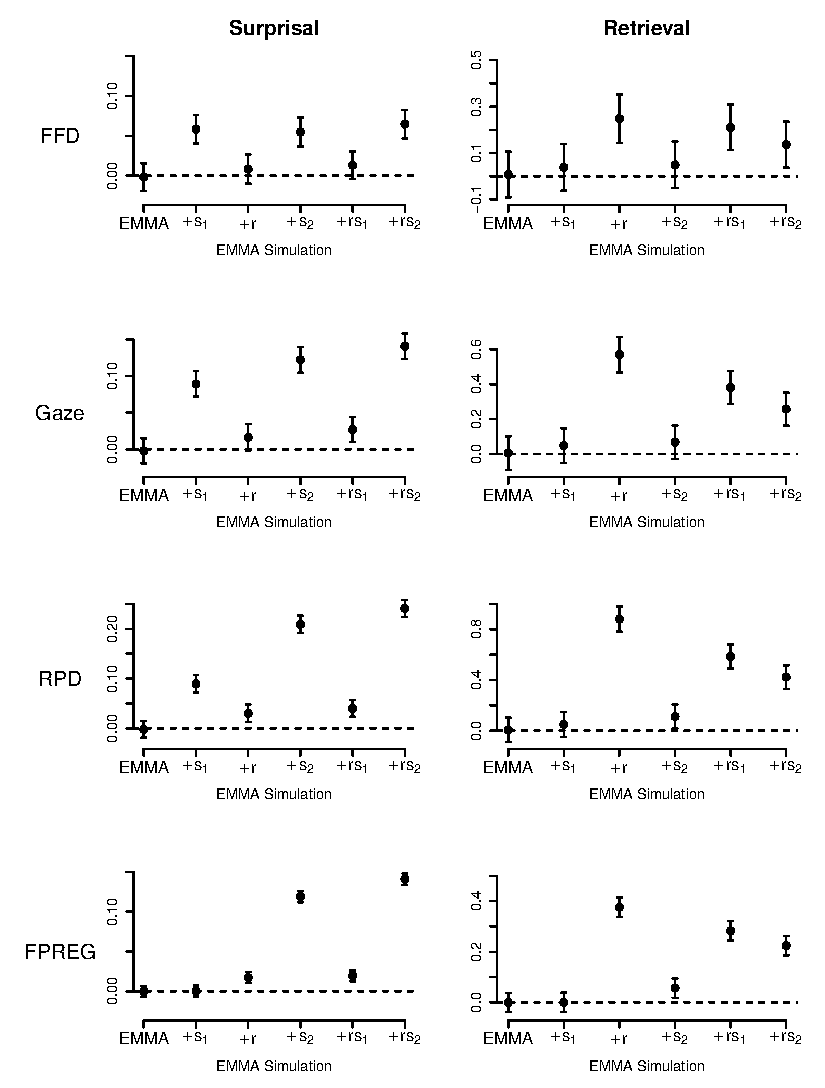
\includegraphics[width=0.8\textwidth]{figures/fig-lms}
\end{center}
\caption{Coefficients and 95\% confidence intervals for predictors surprisal and retrieval estimated by linear regression.  Predictors were log frequency, length, log retrieval, and surprisal.  Coefficients are plotted along the y-axis for surprisal on the left side and retrieval on the right side. Regressions were carried out on the simulated data of all six EMMA models (shown on the x-axis).  95\% confidence intervals that do not cross 0 indicate statistical significance at $\alpha = 0.05.$}
\label{fig:pred}
\end{figure}

\begin{sidewaystable}
%\centering
%\small
\caption{Linear regression results for predictors retrieval and surprisal} \label{lmtable}
\begin{tabular}{llrrrlrrr}
%\toprule
 & & \multicolumn{3}{c}{Model EMMA+rs$_2$} & & \multicolumn{3}{c}{Data (Boston et al., 2011)}  \\ \cline{3-5} \cline{7-9}
% latex table generated in R 2.15.2 by xtable 1.7-0 package
% Tue Nov 27 13:22:29 2012
Measure & Predictor & Coef. & SE & t  / z &   & Coef. & SE & t / z \\ 
%\midrule
SFD & Retrieval & 0.102 & 0.056 & 1.8 &   & 0.00015 & 0.00001 & 18.2 \\ 
    & Surprisal & 0.034 & 0.013 & 2.7 &   & 0.04384 & 0.00200 & 21.9 \\ 
  FFD & Retrieval & 0.136 & 0.051 & 2.7 &   & 0.00016 & 0.00001 & 21.1 \\ 
    & Surprisal & 0.065 & 0.009 & 7.1 &   & 0.05209 & 0.00179 & 29.0 \\ 
  Gaze & Retrieval & 0.258 & 0.049 & 5.3 &   &  &  &  \\ 
    & Surprisal & 0.141 & 0.009 & 16.0 &   &  &  &  \\ 
  TFT & Retrieval & 0.439 & 0.047 & 9.4 &   & 0.00008 & 0.00001 & 8.0 \\ 
    & Surprisal & 0.202 & 0.008 & 23.8 &   & 0.04588 & 0.00239 & 19.2 \\ 
  RPD & Retrieval & 0.422 & 0.048 & 8.9 &   & 0.00010 & 0.00001 & 9.3 \\ 
    & Surprisal & 0.241 & 0.009 & 28.0 &   & 0.05530 & 0.00253 & 21.8 \\ 
  FPREG & Retrieval & 0.224 & 0.020 & 11.4 &   & 0.00026 & 0.00008 & 3.5 \\ 
    & Surprisal & 0.141 & 0.004 & 37.7 &   & 0.16890 & 0.01767 & 9.6 \\ 
%\bottomrule
\end{tabular} \\
{\footnotesize \emph{Notes:} For FPREG z-values are shown, otherwise t-values. FPREG was modelled with a generalized linear model with a binomial link function for EMMA and a generalized linear mixed model by Boston et al. (2011). For all other dependent measures a linear model was used for EMMA's predictions and a linear mixed model by Boston et al.\ (2011).}
\end{sidewaystable}

\end{subappendices}
